\chapter{Metodologia}

\section{Objetivos}

Em resumo, o projeto propõe um sistema embarcado que se comunicará com o usuário por meio de um display LCD 24x2 e microfones. Esse sistema funcionará como uma interface entre o usuário e à AVS. Para isso, esse sistema se comunicará com o AWS IoT Core via protocolo MQTT, serviço responsável pela integração do dispositivo com a AVS. A \autoref{fig_project_diagram} mostra o diagrama de integração do sistema embarcado (dispositivo IoT) à AVS, por meio da tecnologia AWS IoT Core.

\begin{figure}[htb]
	\begin{center}
		\caption{Diagrama de uso dos serviços AWS e da AVS no projeto.}
		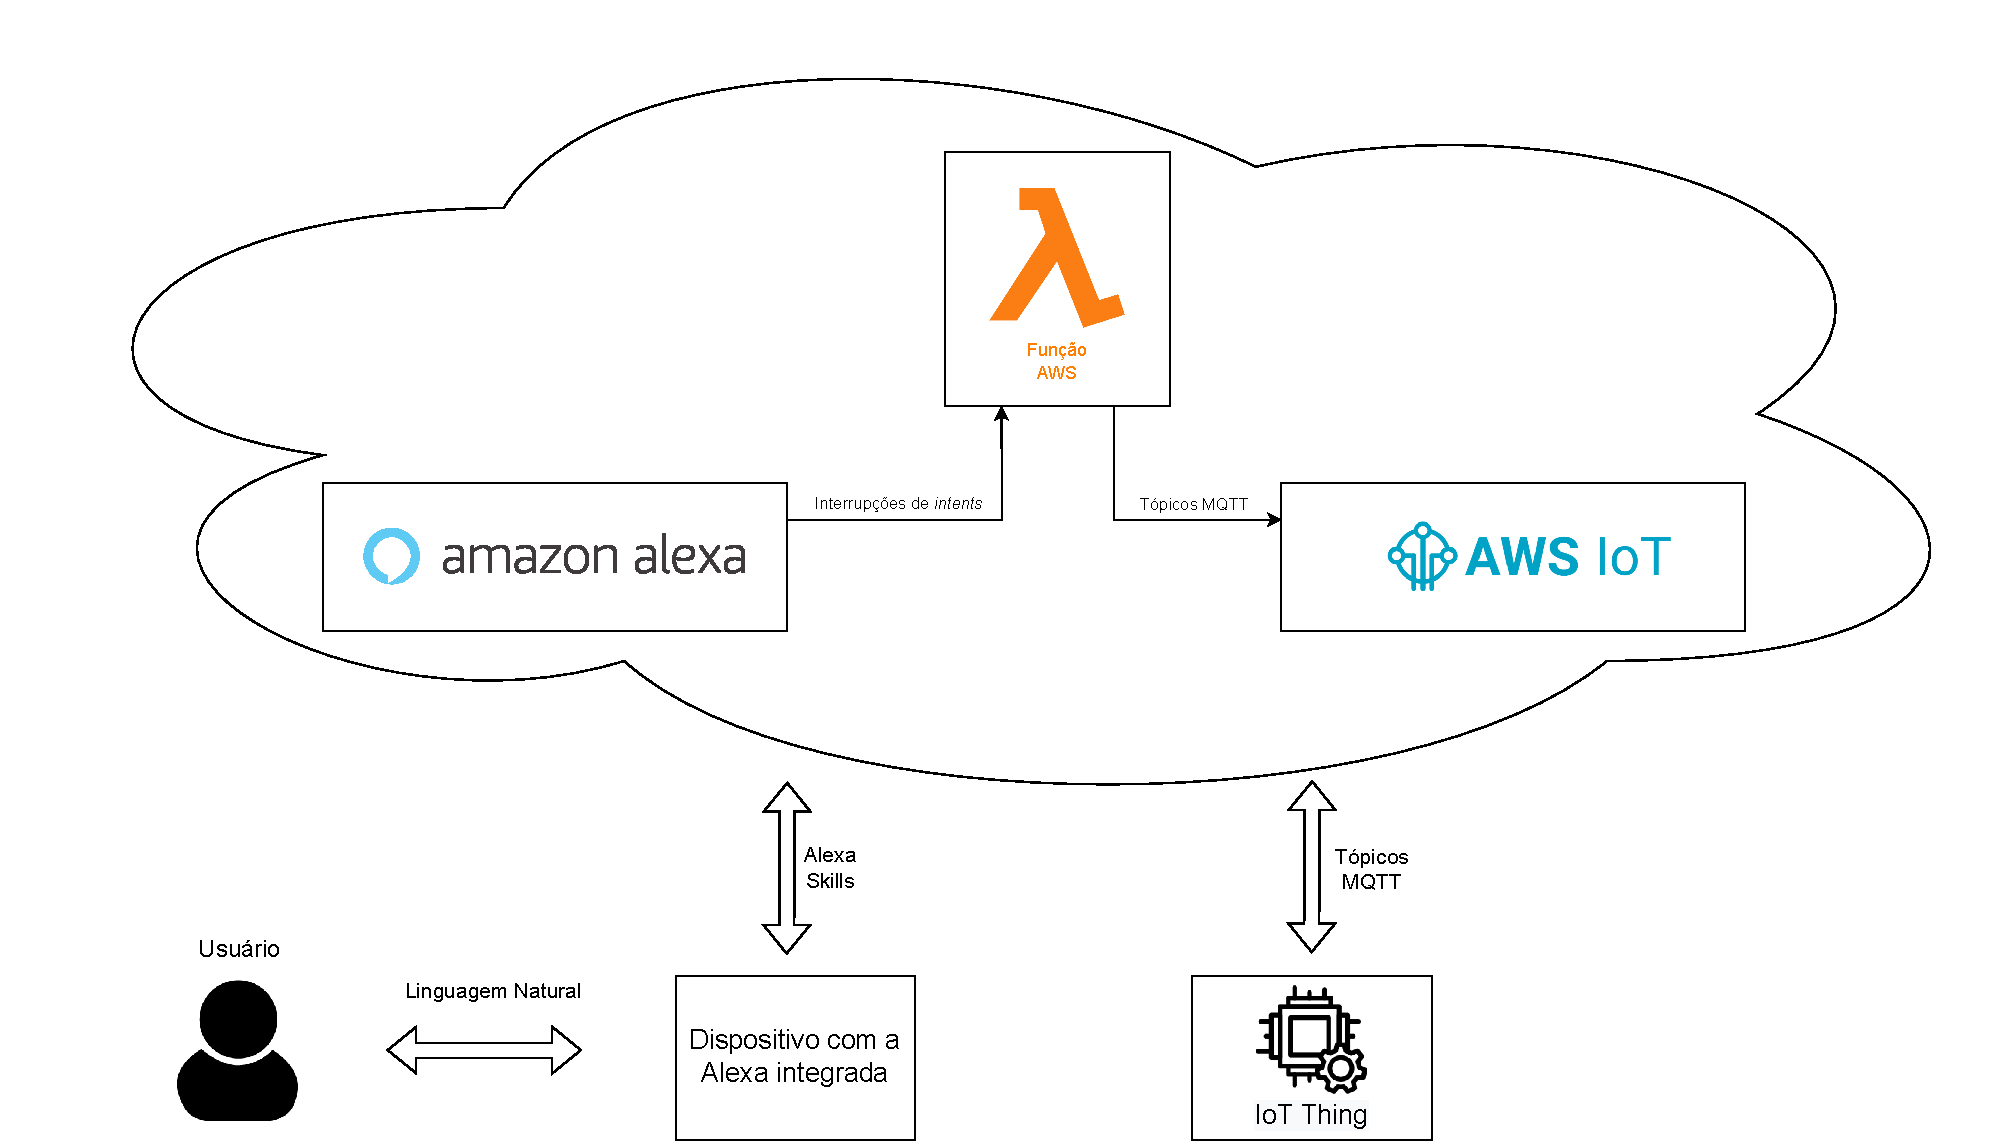
\includegraphics[scale=0.4]{Imagens/project_diagram.pdf}
	\end{center}
	\legend{Fonte: Autor (2022).}
	\label{fig_project_diagram}
\end{figure}

Para esse dispositivo, tem-se os seguintes requisitos funcionais:
\begin{alineas}
	\item Suporte à rede Wifi IEEE 802.11 (2,4 GHz);
	\item Acionamento da Alexa por voz ou toque;
	\item Comunicação do usuário com o dispositivo em linguagem natural, a partir de microfones;
\end{alineas}

A seguir, tem-se os requisitos não-funcionais:
\begin{alineas}
	\item Velocidade (a definir);
	\item Preço (a definir);
	\item Confiabilidade (Como medir isso?);
	\item Capaz de entender o usuário em ambientes ruidosos (Como medir isso?);
\end{alineas}

\section{Projeto de Hardware}
Uma vez escolhidos os requisitos funcionais e não-funcionais do projeto, inicia-se o projeto de hardware. Tomando o baixo custo de produção como um importante requisito do projeto, optou-se pelo uso de sistemas embarcados no protótipo. Computadores e notebooks pessoais, por exemplo, possuem um propósito geral e um alto valor agregado, enquanto um sistema embarcado realiza um conjunto de tarefas predefinidas e normalmente possuem um menor valor agregado (PrimeUP, 2022). Isso posto, inicia-se o estudo dos requisitos de um hardware a ser utilizado em aplicações IoT. Os parâmetros mínimos recomendados pela AWS podem ser vistos na \autoref{table_reduced_hardware_footprint}.

\begin{table}[htb]
	\begin{tblr}{@{}|X[c,valign=m,gray!30]|X[c,valign=m]|@{}}
		\hline
		\textbf{Processador}      & \begin{tabular}[c]{@{}c@{}}ARM M7 or equivalent\\ Arm M4 + AFE DSP\end{tabular} \\ \hline
		\textbf{RAM}              & \begin{tabular}[c]{@{}c@{}}MB for ARM M7\\ 500KB for M4 + AFE DSP\end{tabular}  \\ \hline
		\textbf{Target OS}        & FreeRTOS                                                                        \\ \hline
		\textbf{Conectividade}    & MQTT over Wi-Fi                                                                 \\ \hline
		\textbf{\# de Microfones} & 2+                                                                              \\ \hline
		\textbf{Auto-falante}     & Optimized for speech playback                                                   \\ \hline
	\end{tblr}
	\caption{Parâmetros mínimos recomendados pela AWS para o desenvolvimento de um dispositivo de IoT integrado à AVS.}
	\label{table_reduced_hardware_footprint}
\end{table}

Para a prototipagem, alguns kits de desenvolvimento disponíveis no mercado foram estudados. As tabelas \autoref{table_development_kit_a} e \autoref{table_development_kit_b} mostram informações coletadas de cinco diferentes kits.

Assim como pode ser visto na \autoref{table_reduced_hardware_footprint}, A AWS recomenda o Sistema Operacional FreeRTOS, descartando o \textit{CORE-V MCU DevKit}. Ademais, definiu-se como requisito funcional a comunicação do usuário com o dispositivo através de linguagem natural, demandando no mínimo dois microfones e descartando o \textit{Home Hub 100 Dev Kit for Amazon AVS}. O \textit{STEVAL-VOICE-UI}, embora atenda todos os requisitos funcionais e não-funcionais do projeto e supere os requisitos mínimos sugeridos pela AWS, é somente uma referência de hardware para aplicações IoT. Assim, o esquemático do projeto está disponível no site da STMicroelectronics mas o dispositivo não está disponível para a venda. Como a compra e a soldagem dos componentes individuais demandam tempo e recurso financeiro, a escolha desse dispositivo entra em contraponto à ideia principal de um protótipo: validar uma ideia de maneira fácil, barata e veloz.

Por fim, restando somente os dispositivos \textit{B-L475E-IOT01A2} e \textit{SLN-ALEXA-IOT}, avaliou-se o preço nas lojas oficiais. O primeiro tem o preço de \$51,94, enquanto o segundo \$171,35. Essa discrepância de valores acontece devido à diferença nas especificações: o primeiro dispositivo possui processador Arm® Cortex®-M4, módulo Wi-Fi e dois microfones, enquanto o segundo processador Arm® Cortex®-M7, módulo Bluetooth, módulo Wi-Fi e três microfones. Dessa forma, conclui-se que o dispositivo \textit{B-L475E-IOT01A2} é o dispositivo, com menor custo, que mais se aproxima dos requisitos mínimos especificados pela AWS.

\begin{table}[htb]
	\begin{tblr}{@{}|X[c,valign=m,gray!30]|X[c,valign=m]|X[c,valign=m]|X[c,valign=m]|X[c,valign=m]|X[c,valign=m]|@{}}
		\hline
		\textbf{Número de produto}        & B-L475E-IOT01A2                                                             & CORE-V MCU DevKit                                                   & SLN-ALEXA-IOT                                  \\ \hline
		\textbf{Descrição}                & STM32L4 Discovery kit IoT node, low-power wireless, BLE, NFC, SubGHz, Wi-Fi & European RISC-V chip for IoT development kit                        & EdgeReady MCU Based Solution for Alexa for IOT \\ \hline
		\textbf{Processador}              & Arm® Cortex®-M4                                                             & CV32E40P processor core                                             & Arm® Cortex®-M7 Core                           \\ \hline
		\textbf{FreeRTOS Disponível?}     & Sim                                                                         & Não Disponível                                                      & Sim                                            \\ \hline
		\textbf{Conectividade}            & Inventek ISM43362 Wi-Fi Module                                              & Espressif AWS IoT ExpressLink Module for AWS IoT cloud interconnect & Bluetooth LE 4.2, 802.11 b/g/n Wi-Fi®          \\ \hline
		\textbf{Microfones}               & 2 digital omnidirectional microphones (MP34DT01)                            & Não Disponível                                                      & Digital MEMS microphones (x3)                  \\ \hline
		\textbf{Auto-falante}             & Não Disponível                                                              & Não Disponível                                                      & Não Disponível                                 \\ \hline
		\textbf{Preço nas Lojas Oficiais} & \$53,00                                                                     & Preços Individuais                                                  & \$171,35                                       \\ \hline
	\end{tblr}
	\caption{kits de desenvolvimento recomendados pela Amazon para o desenvolvimento de aplicações IoT (A).}
	\label{table_development_kit_a}
\end{table}

\begin{table}[htb]
	\begin{tblr}{@{}|X[c,valign=m,gray!30]|X[c,valign=m]|X[c,valign=m]|X[c,valign=m]|X[c,valign=m]|X[c,valign=m]|@{}}
		\hline
		\textbf{Número de produto}        & Home Hub 100 Dev Kit for Amazon AVS                                                                                                                                             & STEVAL-VOICE-UI                                                                                                                                                            \\ \hline
		\textbf{Descrição}                & A hardware and software development kit with multi-core connectivity designed to support AVS for AWS IoT Core connected devices                                                 & Qualified hardware reference design enabling easy and cost effective addition of the Alexa Voice Service (AVS) Integration for AWS IoT core to your smart embedded devices \\ \hline
		\textbf{Processador}              & Arm Cortex-M4F CPU                                                                                                                                                              & Dual Arm® Cortex®-A7 and Cortex®-M4 Cores                                                                                                                                  \\ \hline
		\textbf{FreeRTOS Disponível?}     & Sim                                                                                                                                                                             & Sim                                                                                                                                                                        \\ \hline
		\textbf{Conectividade}            & Integrated Bluetooth 5, Qualcomm® Bluetooth Mesh connectivity, low power Wi-Fi 802.11n in 2.4GHz/5GHz bands, and 802.15.4, with support for ZigBee3.0 and Thread via OpenThread & WIFI subsystem including Murata 1DX module used in bypass mode and ISSI IS25LP016D 2Mbytes NOR flash hosting WIFI low level software                                       \\ \hline
		\textbf{Microfones}               & Não Disponível                                                                                                                                                                  & 2 MP23DB01HP Microphone Mems                                                                                                                                               \\ \hline
		\textbf{Auto-falante}             & 1x                                                                                                                                                                              & 1x (8 ohm)                                                                                                                                                                 \\ \hline
		\textbf{Preço nas Lojas Oficiais} & £42.95                                                                                                                                                                          & Não Disponível                                                                                                                                                             \\ \hline
	\end{tblr}
	\caption{kits de desenvolvimento recomendados pela Amazon para o desenvolvimento de aplicações IoT (B).}
	\label{table_development_kit_b}
\end{table}

\section{Projeto de Software}
